\documentclass[a4paper,12pt]{report}
\usepackage{titlesec}
\usepackage{tocloft}
\usepackage{pdfpages}
\usepackage{hyperref}
\usepackage{abstract}
\usepackage{import}
\usepackage{enumitem}
\usepackage[utf8]{inputenc}
\usepackage[T1]{fontenc}
\usepackage[french]{babel} 
\usepackage{xcolor,graphicx}
\newcounter{insertpages}
\usepackage{glossaries}
\graphicspath{{image/}}
\newcommand{\RomanNumeralCaps}[1]
    {\MakeUppercase{\romannumeral #1}}
\definecolor{blue}{RGB}{31,56,100}
\usepackage[top=1cm, bottom=2cm, left=2cm, right=2cm]{geometry}
\linespread{1.5}

\definecolor{blue}{RGB}{31,56,100}
\newenvironment{poliabstract}[1]
  {\renewcommand{\abstractname}{#1}\begin{abstract}}
  {\end{abstract}}



\begin{document}

\renewcommand{\listfigurename}{Table des figures}
\renewcommand{\listtablename}{Table des matières}

\pagenumbering{gobble}


\includepdf[pages={1}]{couverture.pdf}

\null\newpage


\includepdf[pages={1}]{couverture final.pdf}

\input{Remerciements}


\pagenumbering{roman}
 
\null\newpage


\chapter*{}
\addcontentsline{toc}{chapter}{Cahier des charges} 

%minipage pour qu'il n'y ait pas de saut de page à cause d'includepdf

\begin{minipage}{\textwidth}
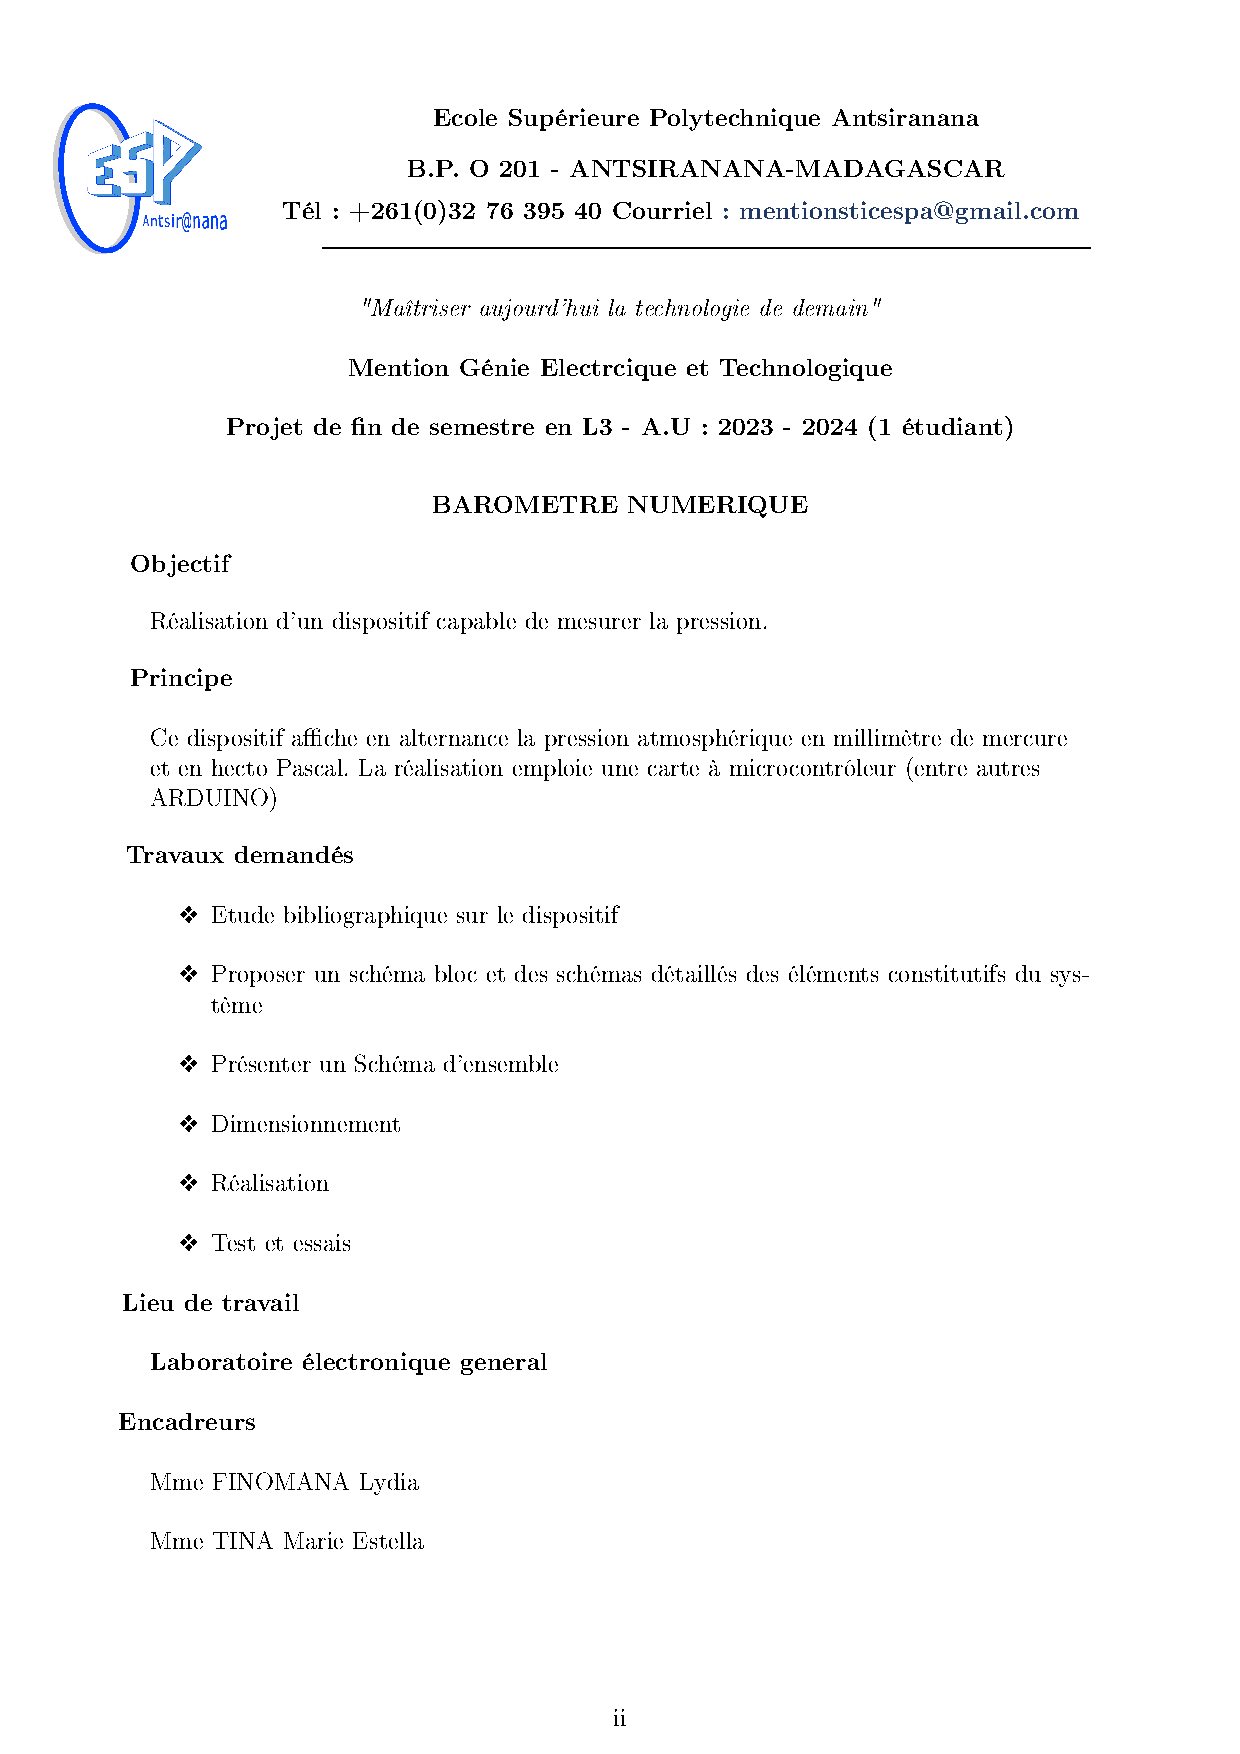
\includepdf[pages={1}]{cahier de charge.pdf}
\end{minipage}

\pagenumbering{roman}
\setcounter{page}{2}




\listoffigures{}


\tableofcontents{}



\chapter*{Résumé}
 

\addcontentsline{toc}{chapter}{Résumé}

	Ce rapport de licence a pour but de montrer un dispositif de mesure météorologique tout en mettant en exergue les problématiques auxquelles il répond et les solutions adéquates. Nous commencerons par introduire la notion de pression, la pression atmosphérique, sa relation avec l'altitude, et les différents instruments de mesure de celle-ci.\\

Après cela, nous établirons la faisabilité du dispositif, nous proposerons sous différents schémas son architecture. Et décrirons les méthodes utilisées, les raisons des choix faits, et appliquées pour lors de sa conception.\\

Enfin, nous présenterons la réalisation du dispositif, les essais et tests, et les différents résultats obtenu.\\       
 


{\let\clearpage\relax\par \vspace{-2cm} 

\chapter*{Abstract}
\addcontentsline{toc}{chapter}{Abstract}

The aim of this report is to demonstrate a meteorological measuring device, highlighting the problems it addresses and the solutions it offers. We'll start by introducing the concept of pressure, the different types of pressure, and its relationship with altitude.\\

After that, we'll establish the feasibility of the device, and propose its architecture in various diagrams. And we'll describe the methods used, the reasons for the choices made and applied in its design.\\

Finally, we will present the realization of the device, the different results obtained, and the different results obtained.  

} %mettre 2 chap sur une même page%

\chapter*{Introduction générale}
\addcontentsline{toc}{chapter}{Introduction générale}
 
	Lorsque l'on veut obtenir des informations météorologiques, ou comprendre pourquoi à un niveau d'altitude donné l'air se raréfie, tout cela nous ramène à la pression.

Celle-ci est étudiée dans des domaines comme la thermodynamique, la mécanique des fluides, la navigation aérienne. De ce fait il est crucial d'améliorer son domaine de mesure.\\

Pendant des siècles la mesure de la pression fait d'énormes avancées mais la précision des résultats étaient pour la plupart aberrant. Mais avec les avancées en électronique, puis l'arrivée de capteurs performant, l'amélioration des instruments de mesures tels l'anémomètre, les altimètres, et enfin le baromètre, ont permis de plus grande plage mesure ainsi qu'une précision plus accrue.\\

Ce travail intitulé "Réalisation et conception d'un baromètre numérique" rentre dans le cadre d'un dispositif à but météorologique seulement. Il en découle, que le dispositif en question sera utilisé pour la collecte de données météo en temps réel.

Ainsi, pour mieux appréhender et analyser les détails de la réalisation et la conception du dispositif, nous avons réparti le travail en 3 parties. La première, qui concerne les généralités sur le baromètre, la pression atmosphériques, et quelques méthodes de mesure de celle-ci. La seconde, concernera l'étude et la conception du baromètre numérique. Finalement, la dernière partie portera sur la réalisation et les essais effectué sur celle-ci.     
    
\pagenumbering{arabic}
\setcounter{page}{1}       






\input{généralités}



\end{document}
